\documentclass{article}
\usepackage{graphicx} % Required for inserting images
\usepackage{float}
\usepackage{amssymb}
\usepackage{amsmath}
\usepackage{amsthm}
\newtheorem{definition}{Definition}
\newtheorem{lemma}{Lemma}
\newtheorem{theorem}{Theorem}
\usepackage[english]{babel}
\usepackage{amsthm}
\usepackage{tikz}
\usepackage{mathtools}
\usetikzlibrary {matrix}
\usepackage{enumitem}% http://ctan.org/pkg/enumitem
\usepackage{caption}
\usepackage{subcaption}
\usepackage{multicol}
\usepackage{multirow}
\usetikzlibrary{arrows}
\usetikzlibrary {arrows.meta}
\usetikzlibrary {calc}
\usepackage{natbib}
\usepackage{xcolor}
\usepackage{tcolorbox}
\usepackage{array}
\usepackage{ctable} % for \specialrule command


\newcolumntype{P}[1]{>{\centering\arraybackslash}p{#1}}

\title{Technical Description: SPLICE: Split-Cloud Experiments for Internet-scale Experimentation }
\author{Cloudflare Research}
\date{August 2024}

\newcolumntype{L}{>{\centering\arraybackslash}m{3cm}}


\begin{document}

\maketitle

\begin{quote}
\textit{\quad All industrial experiments are split-plot experiments.} - Cuthbert Daniel
\end{quote}

\section{Overview}
This document describes the technical details for the Goldilock's challenge page experiments designed as a proof-of-concept of a multifactorial experiment during Innocent's Summer 2024 Research Internship. 
This research and the following experiment design is motivated by the need at Cloudflare to understand the significance of observed effects in the presence of multiple confounding and co-varying phenomena. Passive and active measurements allow the estimation of magnitudes but do very little in supporting our understanding of significance of observed magnitudes especially in the context of a dynamic internal and external computing environment ( for example, load balancing internally and BGP convergence externally). In order to move the needle on practical statistical methods for understanding significance in this context, we leverage split-plot experiment design, a well-understood \textit{design of experiments} design, to develop and implement a first-of-its-kind multi-factorial experiment in the organizational setting of a large content delivery network. Below we describe the design of a \textit{Split-Plot Factorial Experiment with Randomized Complete Blocking and Covariate Adjustment} \cite{Montgomery2020-qa}. We will also refer to the multifactorial design described in this document as a \textit{split-cloud experiment} or a \textit{splice}. In this proof-of-concept, our research questions are:
\begin{enumerate}
    \item What effect do zone type and our traffic load balancing decisions have on the client-perceived request latencies?
    \item Is there a zone type where request latencies perform poorly regardless (or because) of our load balancing decisions?
\end{enumerate}

In the next section, we provide a brief overview of split-plot experiments to motivate our application of the design at Cloudflare


\subsection{What are split-plot experiments?}
\begin{figure}
    \centering
    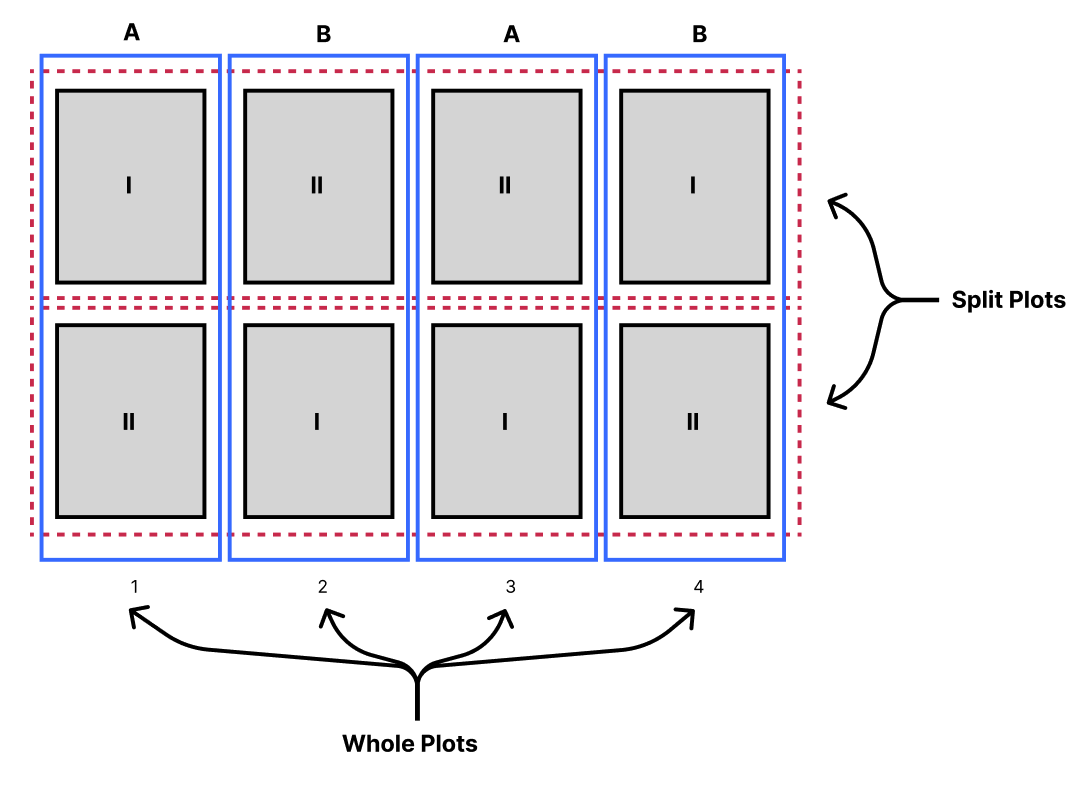
\includegraphics[width=0.8\linewidth]{images/splitplotdesign.png}
    \caption{Split plot experiment layout. Where the whole plot factor has levels \textit{A} and \textit{B} and the split-plot has levels \textit{I} and \textit{II}. The indexes indicate the experimental run. In this example the experiment is replicated twice for each level of the whole plot factor. }
    \label{fig:enter-label}
\end{figure}
Split-plot designs, have their roots in Fisher's work in agricultural experiments and have since become an important factorial DoE tool in industrial setting. 

A split-plot experiment is a blocked experiment design where the blocks are used a experimental units for a subset of factors \cite{Jones2009SplitPlotDW}. In the basic split-plot design, there are two levels of experimental units: the whole plot and the split plot. The whole plots are the blocks and the split plots are the experimental units within a block. The idea of used whole plot as block comes from the understanding that blocking can be used to handle \textit{restrictions on randomization}: these are usually factor that are hard the change between experimental runs. With these two level of experimenal unit we have two different randomization protocols: the first on the whole plot is done to detemine the assigmne to whole plot treatments to whole plots and the second randomizes the split-plot treatments to split-plots within a given block. The key marker for whole and split-plot factors is that whole-plot as mentioned above are usually \textit{hard-to-change} while split-plot factors are \textit{easy-to-change} better runs of the experiments. For a review of split-plot experiments and applications industrual process control, the reader can refer to the following resources: \citealp{Jones2009SplitPlotDW}. 

Split-plots experiments are a type of factorial design and are thus amenable to full and fractional designs. Fractional designs aim to find optimal configurations of a factorial experimental that is equivalent to a full design but which may require a small number of run or meet a constraint on the experiment(er). In this paper we do not focus on optimizing our design, but instead demonstrating the use of split-plot designs in the setting of a global content delivery networks. We call these types of experiments split-cloud experiments or \textit{splices}. In addition to specifying the formal linear model and ANOVA components of our design, we discuss aspects of this design that address particularity of running experiments of this kind on the Internet. 

\subsection{Split-plot experiments @ Cloudflare}

\begin{figure}
    \centering
    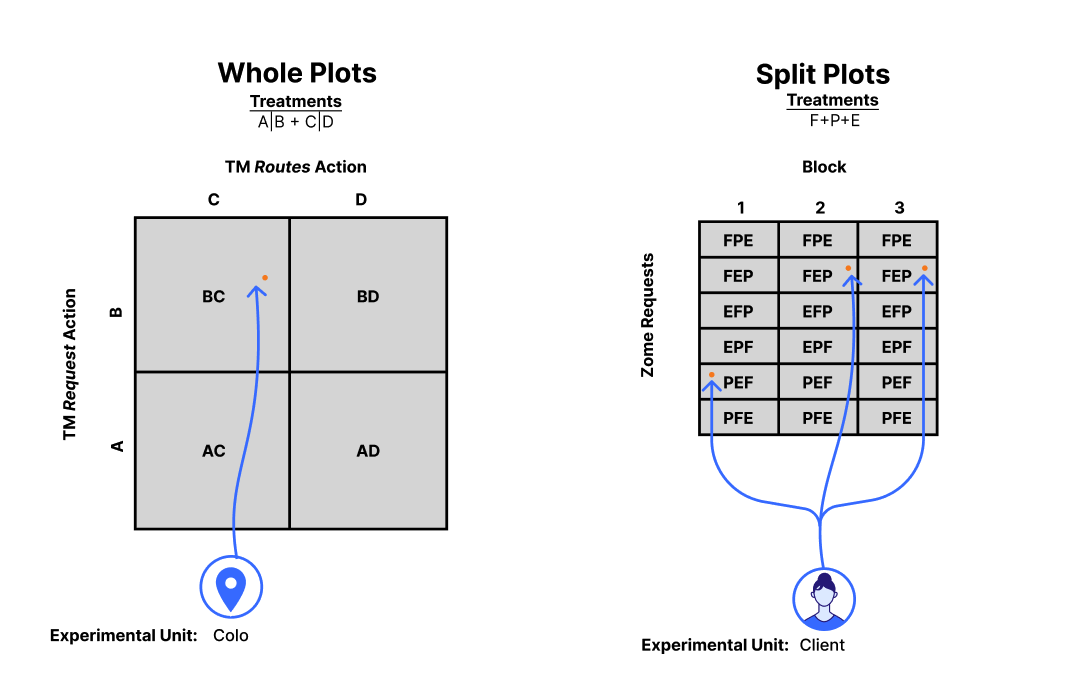
\includegraphics[width=0.8\linewidth]{images/design-split.png}
    \caption{Caption}
    \label{fig:enter-label}
\end{figure}
To understand the model in Equation \ref{eq1}, it is important to understand the two randomization protocols for the two experiments unit in our design:  
\begin{description}
    \item [Protocol 1: ] Cloudflare load balancing strategies which are not `fully randomized' or 'hard-to-change' factors are applied to \textit{whole plots}, which have \textbf{colos} as the experimental unit.
     \item [Protocol 2: ] Client requests to zones are randomized across a number of blocks. Block are sequential and represent the stage in a connection at which the request was initiated. Blocked requests are randomized to subplots which have \textbf{clients} as the experimental unit 
\end{description}

As discussed above, the experimental unit for load balancing decisions is a colocation site or \textit{colo} and the experimental unit for the zones requests is the \textit{client}. This presents a split-plot design where our load balancing decisions are the \textbf{whole-plot factors} and the zone type of the HTTP GET request is the \textbf{split-plot factor}. Our subplot factor ($\mathtt{ZONE}$) has three-levels: $\mathtt{FREE}, \mathtt{PRO}$, and $\mathtt{ENT}$. Our two whole plot factors represent Traffic Manager actions on (1) requests and (2) routes. The first type of action ($\mathtt{TM_{CPU}}$) load balances requests between colos, while the the second action ($\mathtt{TM_{NET}}$) distributes load across network interfaces. For the purpose of simplicity we code these two factors as having only two \textit{levels}: $\mathtt{ACTION}$ or $\mathtt{NO\_ACTION}$. 

We have an additional factor for our blocking that represents the noise associated to TCP Slow Start. The factor is relevant to our subplot effect and thus the experimental unit is also the client. By blocking, we are considering the \textit{nuisance variability} of TCP's congestion window as a \textit{restriction on randomization}. %This means that there are two sources of experimental errors. The first action on the \textit{colo} level and the the second acting on the \textit{client} level.
It is important to note here that blocking is a powerful tool especially when we care about controlling noise of factors that we are not directly interested in. This opens up the possibility of blocking on a number of factors (colo size, region, customer size, etc). Some discretization of these factors in necessary when using full factorial designs and their are benefits to discretization that act as qualitative measures.

\subsection{Effects Model}
\begin{equation} \label{eq1}
\begin{split}
    y_{ijklm} & =  \mu + \tau_{i} + \beta_{j} + \gamma_{k} + (\beta\gamma)_{jk} + \theta_{ijk}  \\
    &  + \phi_m + \delta_{l} + (\beta\delta)_{jl} + (\gamma\delta)_{kl} + (\beta\gamma\delta)_{jkl}
 + \epsilon_{ijklm}
    \begin{cases}
        i = 1,2, \cdots, n \\
        j = 1, 2 \\
        k = 1, 2 \\
        l = 1, 2, 3 \\
        m = 1, 2, \cdots p\\
    \end{cases}
\end{split}
\end{equation}

Formally, our factorial experiment can be described in the \textbf{effects model} in Equation \ref{eq1}. $\tau_{i}$ represent the replication factor (the number of requests),  $\phi_m$ represent the blocking factor effect for TCP slow start, $\beta_{j}$ and $\gamma_k$ represent the whole-plot main effects (Traffic Manager request and routing actions), $\theta_{ijk}$ is the whole-plot error, $\delta_{l}$ represent the subplot main effects (Zone type), and $\epsilon_{ijkl}$ represents the subplot error. The model represents the (main and interaction) effects of four factors: blocks (noise factor controlling for TCP Slow Start), Zone types (with 3 levels), traffic manager request actions, and traffic manager route actions. Right now it assumes the interaction of blocking and treatment is negligible.

\begin{tcolorbox}
\textbf{Note: } If we only consider the whole-plot factor then this would be a completely randomized design with the colos as the experimental units. If we only consider zone type, we could treat the colos as blocks and result in the randomized block design
\end{tcolorbox}


In this proof-of-concept factorial design, we are interested in testing the following basic hypotheses about (1) the equality of sub-plot effects (zone type), 
\begin{equation} \label{eq2}
\begin{split}
    H_0 & : \delta_1 = \delta_2 \cdots \delta_l = 0 \\
    H_1 & : \text{at least one } \delta_i \neq 0
\end{split}
\end{equation}
, (2) the equality of whole-plot (TCP slow start run and traffic manager actions)
\begin{equation} \label{eq3}
\begin{split}
    H_2 & : \beta_1 = \beta_2 \cdots \beta_b = 0 \\
    H_3 & : \text{at least one } \beta_j \neq 0
\end{split}
\end{equation}
\begin{equation} \label{eq4}
\begin{split}
    H_4 & : \gamma_1 = \gamma_2 \cdots \gamma_k = 0 \\
    H_5 & : \text{at least one } \gamma_i \neq 0
\end{split}
\end{equation}
\begin{equation} \label{eq5}
\begin{split}
    H_6 & : \phi_1 = \phi_2 \cdots \phi_h = 0 \\
    H_7 & : \text{at least one } \phi_i \neq 0
\end{split}
\end{equation}
, and (3) the interaction between subplot and whole plot effects (following only demonstrates a single interaction), 
\begin{equation} \label{eq6}
\begin{split}
    H_8 & : (\delta\beta)_{ij} = 0 \ \ \text{for all } i, j \\
    H_9 & : \text{ at least one } (\delta\beta)_{ij} \neq 0
\end{split}
\end{equation}

%\begin{equation} \label{eq2}
%\begin{split}
%    H_0 & : \tau_1 = \tau_2 \cdots \tau_a = 0 \\
%    H_1 & : \text{at least one } \tau_i \neq 0
%\end{split}
%\end{equation}
\subsection{ANOVA Design}
The sum of square for the main effect are found from the totals for each factor as follows:

\begin{table}[t!]
    \centering
    \begin{tabular}{|c|c|c|c|}
        \hline
        \textbf{Plot Type} & \textbf{Symbol} & \textbf{Factor} & \textbf{Description}  \\
        \hline
        \multirow{ 5}{*}{Whole Plot} & $\tau_i$ & Replicates &  \\
        \cline{2-4}
        & $\beta_j$ & $\mathtt{TM_{CPU}}$ & \\
        \cline{2-4}
         &$\gamma_k$ & $\mathtt{TM_{NET}}$ & \\
        \cline{2-4}
        & $\beta_j\gamma_k$ & $\mathtt{TM_{CPU}TM_{NET}}$ & \\
        \cline{2-4}
      & $\theta_{ijk}$ & Whole-plot error & \\
      \hline
      \multirow{ 6}{*}{Split Plot} & $\phi_m$ & Blocks &  \\
        \cline{2-4}
      & $\delta_l$ & $\mathtt{ZONE}$ &\\
      \cline{2-4}
    & $\beta_j\delta_l$ & $\mathtt{TM_{CPU}ZONE}$&  \\
        \cline{2-4}
    & $\gamma_k\delta_l$ & $\mathtt{TM_{NET}ZONE}$ &  \\
      \cline{2-4}
      & $\beta_j\gamma_k\delta_l$ & $\mathtt{TM_{CPU}TM_{NET}ZONE}$ & \\
      \cline{2-4}
      & $\epsilon_{ijklm}$ & Subplot error & \\
      \hline
       \hline
    \end{tabular}
    \caption{Caption}
    \label{tab:my_label}
\end{table}
\begin{table}[h!]
    \def\arraystretch{1.5}
    \centering
    \begin{tabular}{>{\raggedleft}p{3cm} >{\raggedright}p{2cm} P{2cm} c c }
\specialrule{.3em}{.2em}{.2em}
\textbf{Source of Variation} & \textbf{Sum of Squares} & \textbf{Degrees of Freedom} & \textbf{Expected Mean Square} & 
\textbf{F}\\
\specialrule{.1em}{.05em}{.05em} 
    Replicates & $SS_{\text{Replicates}}$ & 
    $(n - 1)$ & $\sigma^{2}_{\epsilon} + 12pn\sum^{2}_{\tau}$ &  \\
     $\mathtt{TM_{CPU}}$ & $SS_{\mathtt{TM_{CPU}}}$ & 1 & $\sigma^{2}_{\epsilon} + 3p\sigma^{2}_{\theta} + 6pn\Sigma_{j=1}^{a}\beta_{j}^{2}$ &\\
      $\mathtt{TM_{NET}}$ & $SS_{\mathtt{TM_{NET}}}$ & 1 & $\sigma^{2}_{\epsilon} + 3p\sigma^{2}_{\theta} + 6pn\Sigma_{k=1}^{b}\gamma_{k}^{2}$ &\\
      $\mathtt{TM_{CPU}TM_{NET}}$ & $SS_{\mathtt{TM_{CPU}TM_{NET}}}$ & 1 & $\sigma^{2}_{\epsilon} + 6p\sigma^{2}_{\theta} + 3pn\sum_{j=1}^{2}\sum_{k=1}^{2}(\beta\gamma)_{jk}^{2}$ & \\
      Whole-plot error & $SS_{\theta}$ & $3(n - 1)$ & $\sigma^{2}_{\epsilon} + 6p\sigma^{2}_{\theta}$ & h \\
      Blocks & $SS_{Blocks}$ & $(p - 1)$ & $\sigma^{2}_{\epsilon} + 12n\sigma^{2}_{\phi}$\\
      $\mathtt{ZONE}$ & $SS_{\mathtt{ZONE}}$ & 2 & $\sigma^{2}_{\epsilon} + 2np\sum_{l=1}^{3}\delta_{l}^{2}$&\\
      $\mathtt{TM_{CPU}ZONE}$ &  $SS_{\mathtt{TM_{CPU}ZONE}}$ & 2 & $\sigma^{2}_{\epsilon} + pn\sum_{j=1}^{2}\sum_{l=1}^{3}(\beta\delta)^{2}_{jl}$&\\
      $\mathtt{TM_{NET}ZONE}$ & $SS_{\mathtt{TM_{NET}ZONE}}$ & 2 & $\sigma^{2}_{\epsilon} + pn\sum_{k=1}^{2}\sum_{l=1}^{3}(\gamma\delta)^{2}_{kl}$&\\
      $\mathtt{TM_{CPU}TM_{NET}ZONE}$ & $SS_{\mathtt{TM_{CPU}TM_{NET}ZONE}}$ & 2 & $\sigma^{2}_{\epsilon} + \frac{np}{2}\sum_{j=1}^{2}\sum_{k=1}^{2}\sum_{l=1}^{3}(\beta\gamma\delta)_{jkl}^{2}$&\\
       Subplot error & $SS_{SP}$ & 
       & & \\
       \hline
       Total & $SS_{T}$ & $(12pn - 1)$ & &\\
    \specialrule{.3em}{.2em}{.2em}
    % $\text{SS}_T - \text{SS}_{Blocks} -\text{SS}_{\mathtt{WP}} - \text{SS}_{\mathtt{ZONE}} - \text{SS}_{\mathtt{TM_{CPU}}\mathtt{ZONE}} - \text{SS}_{\mathtt{TM_{NET}}\mathtt{ZONE}} -\text{SS}_{\mathtt{TM_{NET}}\mathtt{TM_{CPU}}\mathtt{ZONE}}$
\end{tabular}
      \caption{ANOVA for Split-Plot Deign with Blocking, and, Factors in Whole-plot and Factor $\mathtt{ZONE}$ in Subplot}
      \label{tab:anova}
\end{table}


If this assumption is untrue, then we will want to add interaction effects. In Table \ref{tab:anova}, we present the ANOVA components for this design. In the table we use, $\sigma_{\theta}^{2}$ and $\sigma_{\epsilon}^{2}$ represent the variances of the whole-plot and subplit error, respectively. $\sigma_{\tau}^{2}$ is the variance of the block effects. Capital latin letter represent fixed effects. The whole-plot main effects and interaction are tested against the subplot error. If some of the design factors are random then either the test statistic changes or we use Satterthwaite's procedure where this is no exact $F$ test.\\


\subsection{Power Calculation}

\appendix

\section{Sum of Squares for Experiment}

\begin{equation}
    SS_T = \sum_{i=1}^{n}\sum_{j=1}^{2}\sum_{k=1}^{2} \sum_{l=1}^{3}\sum_{m=1}^{p} y^{2}_{ijklm} - \frac{y^{2}_{.....}}{12pn}
\end{equation}

\begin{equation}
    SS_{\mathtt{TM_{NET}}} = \frac{1}{6pn}\sum_{j=1}^{2}y_{.j...}^2 - \frac{y^{2}_{.....}}{12pn}
\end{equation}
\begin{equation}
    SS_{\mathtt{TM_{CPU}}} = \frac{1}{6pn}\sum_{k=1}^{2}y_{..k..}^2 - \frac{y^{2}_{.....}}{12pn}
\end{equation}

\begin{equation}
    SS_{\mathtt{TM_{NET}TM_{CPU}}} = \frac{1}{3pn}\sum_{j=1}^{2}\sum_{k=1}^{2}y_{.jk..}^2 - \frac{y^{2}_{.....}}{12pn} - SS_{\mathtt{TM_{NET}}} - SS_{\mathtt{TM_{CPU}}}
\end{equation}

\begin{equation}
    SS_{WP} = \frac{1}{3p}\sum_{i=1}^{n}\sum_{j=1}^{2}\sum_{k=1}^{2}y_{ijk..}^2 - \frac{y^{2}_{.....}}{12pn}
\end{equation}
\begin{equation}
    SS_{Blocks} = \frac{1}{12n}\sum_{m=1}^{p}y_{....m}^2 - \frac{y^{2}_{.....}}{12pn}
\end{equation}

\begin{equation}
    SS_{\mathtt{ZONE}} = \frac{1}{4pn}\sum_{l=1}^{3}y_{...l.}^2 - \frac{y^{2}_{.....}}{12pn}
\end{equation}

\begin{equation}
    SS_{\mathtt{TM_{NET}ZONE}} = 
    \frac{1}{2pn}\sum_{j=1}^{2}\sum_{l=1}^{3} y_{.j.l.}^{2} - \frac{y^{2}_{.....}}{12pn} - SS_{\mathtt{TM_{NET}}} -  SS_{\mathtt{ZONE}}
\end{equation}

\begin{equation}
    SS_{\mathtt{TM_{CPU}ZONE}} = 
    \frac{1}{2pn}\sum_{k=1}^{2}\sum_{l=1}^{3} y_{..kl.}^{2} - \frac{y^{2}_{.....}}{12pn} - SS_{\mathtt{TM_{CPU}}} -  SS_{\mathtt{ZONE}} 
\end{equation}

\begin{equation}
\begin{split}
    SS_{\mathtt{TM_{CPU}TM_{NET}ZONE}}  = \frac{1}{pn}&\sum_{j=1}^{2}\sum_{k=1}^{2}\sum_{l=1}^{3} y_{.jkl.}^{2} - \frac{y^{2}_{.....}}{12pn} - SS_{\mathtt{TM_{NET}}} - SS_{\mathtt{TM_{CPU}}} \\ 
    &  - SS_{\mathtt{ZONE}} -  SS_{\mathtt{TM_{NET}ZONE}} -  SS_{\mathtt{TM_{CPU}ZONE}}
\end{split}
\end{equation}

\begin{equation}   SS_{SP} = \text{Subtraction}
\end{equation}

\section{Fixed effects : Expected means square treatment sum of squares}
\[
    MS_{\text{Treatments}} = \frac{SS_{\text{Treatments}}}{a - 1}
\]

\begin{equation}
    \begin{split}
        E(MS_{\text{Treatments}}) & = E (\frac{SS_{\text{Treatments}}}{a - 1}) \\ 
        & = \frac{1}{a - 1}E\left[\sum_{i=1}^{a}\sum_{j=1}^{n}(\overline{y}_{i.} - \overline{y}_{..})^2\right] \\
        & = \frac{1}{a - 1}E\left[\sum_{i=1}^{a}\sum_{j=1}^{n} (\overline{y}_{i.}^2 - 2\overline{y}_{i.}\overline{y}_{..} + \overline{y}_{..}^{2})\right]\\
        & = \frac{1}{a - 1}E\left[\sum_{i=1}^{a}\sum_{j=1}^{n}\overline{y}_{i.}^2 - 2\sum_{i=1}^{a}\sum_{j=1}^{n}\overline{y}_{i.}\overline{y}_{..} + \sum_{i=1}^{a}\sum_{j=1}^{n}\overline{y}_{..}^{2}\right] \\
        & = \frac{1}{a - 1}E\left[n\sum_{i=1}^{a}\overline{y}_{i.}^2 - 2an\overline{y}_{..}^2 + an\overline{y}_{..}^{2}\right] \\
        & = \frac{1}{a - 1}E\left[n\sum_{i=1}^{a}\overline{y}_{i.}^2 - an\overline{y}_{..}^{2}\right] \\
        & = \frac{1}{a - 1}E\left[\frac{1}{n}\sum_{i=1}^{a}y_{i.}^2 - \frac{1}{an}y_{..}^{2}\right] \\
        & = \frac{1}{a - 1}E\left[\frac{1}{n}\sum_{i=1}^{a}\left[\sum_{j=1}^{n}(\mu + \tau_{i} + \epsilon_{ij})\right]^2 - \frac{1}{an}\left[ \sum_{i=1}^{a}\sum_{j=1}^{n}(\mu + \tau_i + \epsilon_{ij})\right]^2\right] \\
        & = \frac{1}{a - 1}E\left[\frac{1}{n}\sum_{i=1}^{a}\left[(n\mu)^2 + (n\tau_{i})^2 + \epsilon_{i.}^2)\right] - \frac{1}{an}\left[ (an\mu)^2 + n^2(\sum_{i=1}^{a}\tau_i)^2 + \epsilon_{..}^2)\right]\right] \\
        & = \frac{1}{a - 1}E\left[\frac{1}{n}\left[a(n\mu)^2 + (n^2\sum_{i=1}^{a}\tau_{i}^2) + an\sigma^2)\right] - \frac{1}{an}\left[ (an\mu)^2 + an\sigma^2)\right]\right] \\
        & = \frac{1}{a - 1}E\left[an(\mu^2) + n\sum_{i=1}^{a}\tau_{i}^2 + a\sigma^2 - an(\mu^2) - \sigma^2\right] \\
        & = \frac{1}{a - 1}E\left[ n\sum_{i=1}^{a}\tau_{i}^2 + a\sigma^2 - \sigma^2\right] \\
        & = \frac{1}{a - 1}E\left[ n\sum_{i=1}^{a}\tau_{i}^2 + (a - 1)\sigma^2\right] \\
         & = \frac{n\sum_{i=1}^{a}\tau_{i}^2}{a - 1} + \sigma^2 \\
    \end{split}
\end{equation}


\section{Random effects : Expected means square treatment sum of squares}
\begin{equation}
    \begin{split}
        E(MS_{\text{Treatments}}) & = E (\frac{SS_{\text{Treatments}}}{a - 1}) \\ 
        & = \frac{1}{a - 1}E\left[\sum_{i=1}^{a}\sum_{j=1}^{n}(\overline{y}_{i.} - \overline{y}_{..})^2\right] \\
        & = \frac{1}{a - 1}E\left[\sum_{i=1}^{a}\sum_{j=1}^{n} (\overline{y}_{i.}^2 - 2\overline{y}_{i.}\overline{y}_{..} + \overline{y}_{..}^{2})\right]\\
        & = \frac{1}{a - 1}E\left[\sum_{i=1}^{a}\sum_{j=1}^{n}\overline{y}_{i.}^2 - 2\sum_{i=1}^{a}\sum_{j=1}^{n}\overline{y}_{i.}\overline{y}_{..} + \sum_{i=1}^{a}\sum_{j=1}^{n}\overline{y}_{..}^{2}\right] \\
        & = \frac{1}{a - 1}E\left[n\sum_{i=1}^{a}\overline{y}_{i.}^2 - 2an\overline{y}_{..}^2 + an\overline{y}_{..}^{2}\right] \\
        & = \frac{1}{a - 1}E\left[n\sum_{i=1}^{a}\overline{y}_{i.}^2 - an\overline{y}_{..}^{2}\right] \\
        & = \frac{1}{a - 1}E\left[\frac{1}{n}\sum_{i=1}^{a}y_{i.}^2 - \frac{1}{an}y_{..}^{2}\right] \\
        & =\frac{1}{a - 1}E\left[\frac{1}{n}\sum_{i=1}^{a}\left[\sum_{j=1}^{n}(\mu + \tau_{i} + \epsilon_{ij})\right]^2 - \frac{1}{an}\left[ \sum_{i=1}^{a}\sum_{j=1}^{n}(\mu + \tau_i + \epsilon_{ij})\right]^2\right] \\
        & = \frac{1}{a - 1}E\left[\frac{1}{n}\sum_{i=1}^{a}\left[(n\mu)^2 + (n\tau_{i})^2 + \epsilon_{i.}^2)\right] - \frac{1}{an}\left[ (an\mu)^2 + n^2(\sum_{i=1}^{a}\tau_i)^2 + \epsilon_{..}^2)\right]\right] \\
        & = \frac{1}{a - 1}E\left[\frac{1}{n}\left[a(n\mu)^2 + an^2\sigma^{2}_{\tau} + an\sigma^2\right] - \frac{1}{an}\left[ (an\mu)^2 - an^2\sigma^{2}_{\tau} - an\sigma^2\right]\right]\\
        & = \frac{1}{a - 1}E\left[ (a - 1)n\sigma^{2}_{\tau} + (a - 1)\sigma^2\right]\\
        & =  n\sigma^{2}_{\tau} + \sigma^2
    \end{split}
\end{equation}

\bibliographystyle{acm}
\begin{small}
\bibliography{ref}
\end{small}
\end{document}
